\documentclass[class=beamer, xcolor=dvipsnames, hyperref=hidelinks, preview]{standalone}

%\usepackage[dvipsnames]{xcolor}
%\usepackage[hidelinks]{hyperref}
\usepackage{tikz}
\usetikzlibrary{fit, backgrounds, positioning, shadows, shadows.blur}

\tikzset{portrait/.style={draw, inner sep=0, drop shadow, on grid}}

\begin{document}

\begin{tikzpicture}[node distance=3cm and 3.5cm]
	\node[portrait, label=below:Bjarne Hiller] (hiller) {
		\href{https://bckrlab.org/people/team/bjarne-hiller/}{
\includegraphics[width=2cm]{team/bjarne-hiller.jpg}}
	};

	\node[portrait, label=below:Martin Becker, right=of hiller] (becker) {
		\href{https://bckrlab.org}{
\includegraphics[width=2cm]{team/martin-becker.jpg}}
	};


	\node[portrait, label=below:Sebastian Bader, below=of hiller] (bader) {
		\href{https://www.mmis.informatik.uni-rostock.de/}{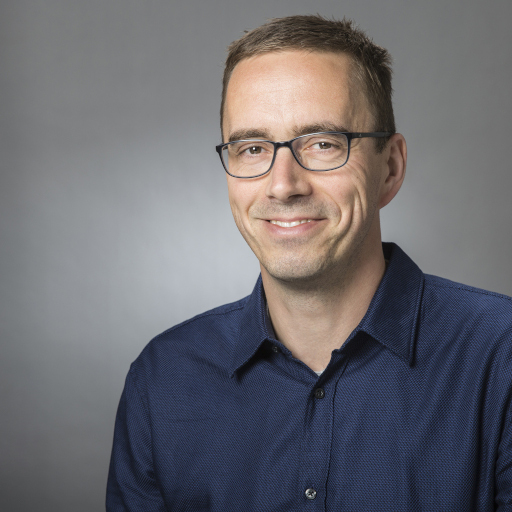
\includegraphics[width=2cm]{team/sebastian-bader.jpg}}
	};

	\node[portrait, label=below:Thomas Kirste, below=of becker] (kirste) {
		\href{https://www.mmis.informatik.uni-rostock.de/}{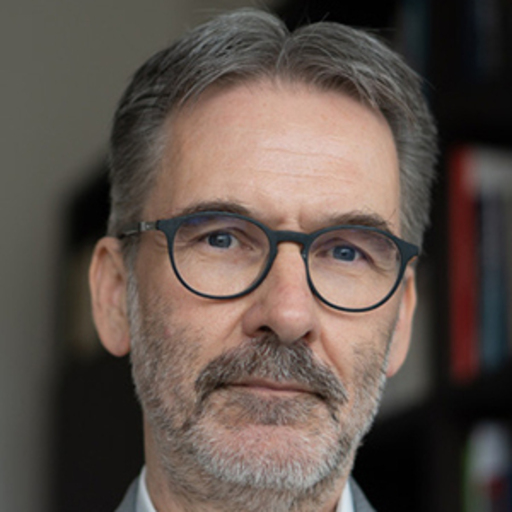
\includegraphics[width=2cm]{team/thomas-kirste.jpg}}};

	\begin{scope}[on background layer]
		\node[fit=(hiller)(kirste), rectangle, fill=Blue!40, inner sep=0.5cm, drop shadow, label=above:University of Rostock] (vac) {};
	\end{scope}

	\node[portrait, label=below:Martin Dyrba, right=of becker] (dyrba) {
		\href{https://explaination.net/}{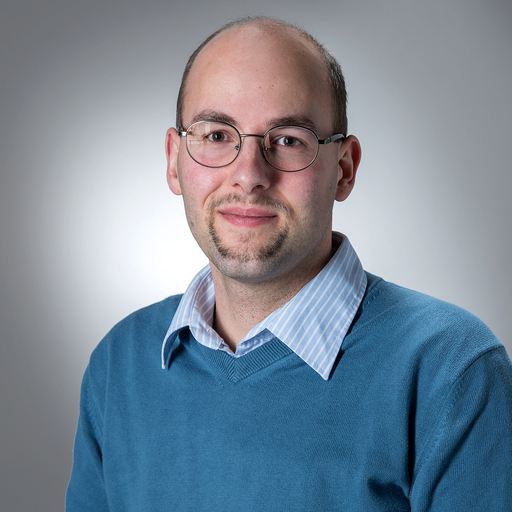
\includegraphics[width=2cm]{team/martin-dyrba.jpg}}
	};

	\node[portrait, label=below:Devesh Singh, below=of dyrba] (singh) {
		\href{https://www.linkedin.com/in/deveshsingh0016/}{
\includegraphics[width=2cm]{team/devesh-singh.jpg}}
	};

	\begin{scope}[on background layer]
		\node[fit=(dyrba)(singh), fill=Orange!20, rectangle, inner sep=0.5cm, drop shadow, label=above:DZNE] (dzne) {};
	\end{scope}

	\node[left=0.5cm of vac.west] {
		\href{https://vac.uni-rostock.de/}{
\includegraphics[width=2cm]{../../../logos/logo-vac}}
	};

	\node[right=0.5cm of dzne.east] {
		\href{https://www.dzne.de/}{
\includegraphics[width=2cm]{../../../logos/logo-dzne}}
	};



\end{tikzpicture}
\end{document}